% Thesis defense — 20 minutes
% Build: latexmk -pdf defense.tex   (from Thesis tex/defense/)
\documentclass[aspectratio=169,10pt]{beamer}

\usetheme{metropolis}
\metroset{sectionpage=progressbar, numbering=fraction, progressbar=frametitle}

\usepackage[english]{babel}
\usepackage[utf8]{inputenc}
\usepackage{booktabs}
\usepackage{amsmath}
\usepackage{graphicx}
\graphicspath{{../img/gen/}{../img/}}

\newcommand{\bcombo}{\texttt{best-combo}}
\newcommand{\good}[1]{\textcolor{green!50!black}{#1}}
\newcommand{\bad}[1]{\textcolor{red!70!black}{#1}}

\title{Hardware-Conscious Performance Engineering of Fainder for Distribution-Aware Dataset Search}
\subtitle{Master's Thesis Defense}
\author{Tarik Abu Mukh}
\institute{Technische Universit\"at Berlin \\ Chair of Database Systems and Information Management (DIMA)\\[1ex]
Reviewers: Prof.\ Dr.\ Volker Markl, Prof.\ Dr.\ Matthias B\"ohm \quad Advisor: Lennart Behme}
\date{\today}

\begin{document}

\maketitle

% ---------------------------------------------------------------- 1. Context
\section{Problem}

\begin{frame}{Distribution-Aware Dataset Search and Fainder}
  \begin{itemize}
    \item Setting: search over millions of datasets where raw data is not accessible (privacy, licensing) --- only per-column \textbf{histograms} are published.
    \item Predicate class: \emph{``find all columns where the $p$-th percentile exceeds threshold $t$.''}
    \item \textbf{Fainder} [Behme et al., VLDB 2024]: an index for this problem.
    \begin{itemize}
      \item K-means clusters histograms, aligns each cluster onto a shared bin grid.
      \item Precomputed cumulative densities $\Rightarrow$ percentile predicates become \textbf{binary search}.
      \item On GitTables (5M histograms): $>$2 orders of magnitude over profile scan, index shrinks from $>$1\,TB to 3.2\,GB.
    \end{itemize}
    \item This thesis: how do we execute Fainder's \emph{query phase} efficiently on a modern multi-core server?
  \end{itemize}
\end{frame}

\begin{frame}{The Problem: Python Runs the Interpreter, Not the Algorithm}
  \begin{columns}[T]
    \column{0.55\textwidth}
    \begin{itemize}
      \item Reference implementation: Python + NumPy.
      \item \textbf{GIL} serialises the per-cluster loop --- wall time is \emph{flat} across all thread counts (2\% spread).
      \item AoS layout pollutes cache lines with unread hist-id fields.
      \item Per-iteration interpreter dispatch compounds onto both.
    \end{itemize}
    \column{0.42\textwidth}
    \begin{block}{10{,}000 queries, 5M histograms}
      \centering
      \Large $\sim$2.4 hours \\[0.5ex]
      \normalsize (8{,}589\,s, any thread count)
    \end{block}
    \begin{itemize}
      \item Interactive exploration untenable.
    \end{itemize}
  \end{columns}
  \vfill
  \begin{itemize}
    \item Curious detail: Python's IPC is \emph{higher} than Rust's (2.35 vs 0.96) --- it retires $6.2\times$ the instructions on bookkeeping. The win is fewer instructions on more cores, not better IPC.
  \end{itemize}
\end{frame}

\begin{frame}{Goal, Scope, Approach}
  \begin{itemize}
    \item \textbf{Goal:} close the gap between Fainder's algorithmic potential and what its implementation achieves --- without changing results.
    \item \textbf{Approach:} re-implement the query phase in \textbf{Rust} (PyO3 extension, same Python API), then run an ablation study across $>$20 hardware-conscious optimisation axes.
    \item \textbf{Hard constraint:} bitwise-identical results to the reference on all workloads (precision $=$ recall $=$ 1.000).
    \item \textbf{Out of scope:} algorithm changes, GPU, distributed execution.
  \end{itemize}
  \vfill
  \begin{alertblock}{The core of the thesis is the investigation, not the port}
    Four binding hardware ceilings, a negative-composability pattern across five axes, and a pre-flight methodology that follows from it.
  \end{alertblock}
\end{frame}

% ---------------------------------------------------------------- 2. Method
\section{Method}

\begin{frame}{Experimental Setup}
  \textbf{Hardware} (representative of a search-service deployment node):
  \begin{itemize}
    \item 2$\times$ Intel Xeon Platinum 8468H (Sapphire Rapids), 96 physical / 192 logical cores.
    \item 105\,MiB L3 per socket, 1\,TB DDR5-4800, UPI cross-socket ($\sim$2.1$\times$ remote-load penalty).
  \end{itemize}
  \textbf{Workloads} (GitTables, 10K percentile queries shared across all):
  \begin{center}
    \small
    \begin{tabular}{lrrrl}
      \toprule
      Dataset & $n_\text{hists}$ & $K_\text{eff}$ & hists/cluster & role \\
      \midrule
      \texttt{c256\_10gb}  & 324\,K  & 129 & $\sim$2.5\,K & small \\
      \texttt{c256\_30gb}  & 997\,K  & 184 & $\sim$5.4\,K & medium \\
      \texttt{c256\_56gb}  & 5.02\,M & 191 & $\sim$26\,K  & \textbf{primary} \\
      \texttt{c1024\_56gb} & 5.02\,M & 610 & $\sim$8.2\,K & out-of-distribution \\
      \bottomrule
    \end{tabular}
  \end{center}
  \textbf{Protocol:} 5-rep medians, thread sweep $t \in \{1 \dots 96\}$, \texttt{perf} counters per cell, warm cache, suppress-results vs with-results separated. All claims trace to a benchmark database (2{,}658 runs).
\end{frame}

\begin{frame}{The Rust Engine}
  \begin{itemize}
    \item Query engine as a compiled extension module (PyO3 + Maturin); clustering and loading stay in Python.
    \item Rayon work-stealing parallelism over clusters; no GIL in the hot path.
    \item Optimisation axes as Cargo feature flags, so every variant is a separate measurable build:
    \begin{itemize}
      \item \textbf{Layout:} SoA vs AoS, f16 half-precision, Eytzinger, packed IDs, per-cluster reindexing.
      \item \textbf{Search:} AVX-512 SIMD leaf stage, 8-way batch, horizontal lockstep, PGM learned index.
      \item \textbf{Scheduling:} column-centric engine, query-batch, morsel-driven scheduler, core pinning.
      \item \textbf{Memory:} pooled output buffers, mimalloc, NUMA placement.
    \end{itemize}
    \item Rebinning (index construction) also ported: one fused parallel kernel per cluster.
    \item Every build validated bitwise-identical to the Python reference.
  \end{itemize}
\end{frame}

% ---------------------------------------------------------------- 3. Results
\section{Results: Four Ceilings}

\begin{frame}{Finding 1: Four Performance Ceilings}
  \begin{columns}[T]
    \column{0.60\textwidth}
    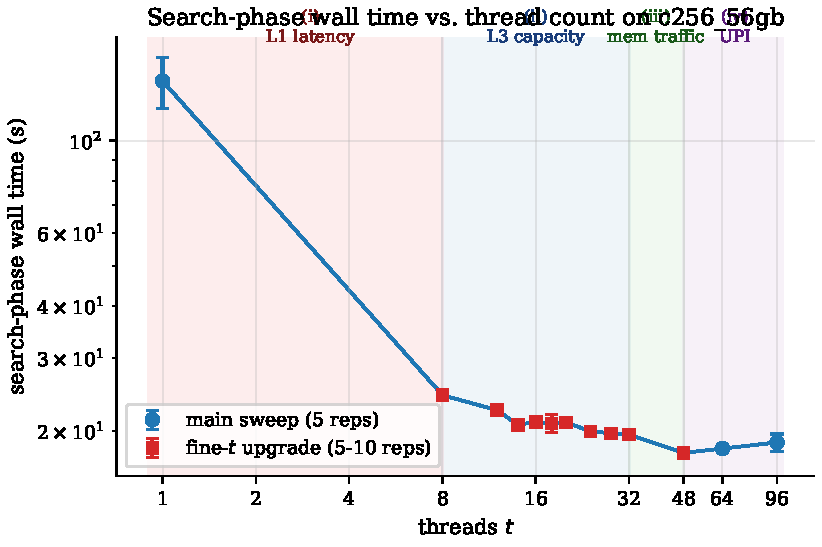
\includegraphics[width=\linewidth]{ch4_four_ceilings.pdf}
    \column{0.38\textwidth}
    \small
    \begin{enumerate}
      \item \textbf{Compute / L1 latency} ($t \leq 8$) --- candidate, \bad{refuted}.
      \item \textbf{Shared L3 capacity} ($t \approx 16$).
      \item \textbf{On-socket memory-traffic pressure} ($t \in [32,48]$).
      \item \textbf{Cross-socket UPI} ($t > 48$).
    \end{enumerate}
    \vfill
    Each binds in a different regime; each responds to a different class of interventions.
  \end{columns}
\end{frame}

\begin{frame}{Ceiling (i): The Literature's Default --- Refuted Here}
  \begin{itemize}
    \item Binary search is a serial dependent-load chain; the default assumption is that load latency is the wall.
    \item Four latency-side ablations, all \textbf{null or marginal} ($0.90$--$1.13\times$ across all cells):
    \begin{itemize}
      \item AVX-512 leaf-stage SIMD
      \item 8-way pipelined batch-search
      \item 16-query horizontal-SIMD lockstep
      \item PGM learned index
    \end{itemize}
    \item Why: the bin-boundary array ($\sim$142 entries) sits in two L1d lines; the column slice is L2-resident. The chain is short and cache-friendly --- there is no latency headroom to recover.
  \end{itemize}
  \vfill
  \begin{alertblock}{A refutation is a finding}
    On this workload and hardware, no latency-side intervention moves the wall. The action is all above L1.
  \end{alertblock}
\end{frame}

\begin{frame}{Ceiling (ii): Shared L3 --- Two Mechanisms, Not One}
  \begin{itemize}
    \item \texttt{pooled} (pre-allocated output buffers): \good{$-46.9\%$} at $t{=}1$, \good{$-34.1\%$} at $t{=}8$, \good{$-20.2\%$} at $t{=}16$ on the primary workload.
    \begin{itemize}
      \item Binding mechanism at moderate $t$: \textbf{glibc allocator-arena mutex}, not raw L3 capacity.
    \end{itemize}
    \item \texttt{f16} (halved footprint): \textbf{no standalone win} on the primary workload; inside the bundle it is a \bad{$+15.6\%$ drag} at $t{=}16$.
    \begin{itemize}
      \item Same feature on the sparser OOD workload: \good{saves $20.9\%$} inside the bundle.
      \item Sign flips with cluster density --- footprint halving only pays when it unlocks a new cache-resident regime.
    \end{itemize}
    \item AoS negative control: $+17\%$ penalty at $t{=}8$, flips to $-4\%$ at $t{=}64$ --- the binding ceiling itself moves with $t$.
  \end{itemize}
  \vfill
  Ceiling (ii) = arena-mutex serialisation on dense clusters, aggregate L3 footprint on sparse ones.
\end{frame}

\begin{frame}{Ceilings (iii) and (iv): Memory Traffic and the Socket Boundary}
  \textbf{Ceiling (iii): on-socket memory-traffic pressure} ($t \in [32,48]$)
  \begin{itemize}
    \item Anti-scaling: wall time \emph{rises} as cores are added.
    \item Not ``DRAM bandwidth'': measured traffic is a small fraction of STREAM peak. Pressure, not saturation.
    \item Interventions that reduce bytes per comparison / per emitted result apply here.
  \end{itemize}
  \vfill
  \textbf{Ceiling (iv): cross-socket UPI} ($t > 48$)
  \begin{itemize}
    \item Separated from (iii) by a four-configuration \texttt{numactl} probe.
    \item Single-socket placement saves \good{11--13\%} at $t \leq 48$.
    \item Page-granular interleave across sockets \bad{regresses $+26$--$41\%$}: 4\,KB round-robin defeats the prefetcher.
  \end{itemize}
\end{frame}

% ---------------------------------------------------- 4. Structural finding
\section{Results: Negative Composability}

\begin{frame}{Finding 2: Optimisations Compose Negatively}
  Five ablation pairs, five different hardware axes, one shape: \emph{the coarser optimisation already absorbed the headroom; the finer one's overhead becomes net cost.}
  \begin{center}
    \small
    \begin{tabular}{llr}
      \toprule
      Composition & Intended axis & Outcome \\
      \midrule
      \bcombo{} $+$ \texttt{packed-ids} & emit-ID bandwidth & \bad{NEG} 12/18 cells, up to $+24\%$ \\
      \bcombo{} $+$ qbatch $K{=}128$ & cold-load amortisation & \bad{NEG} every cell, $+8$ to $+32\%$ \\
      qbatch $+$ morsel & cross-worker coordination & \bad{NEG} every cell, $+8$ to $+12\%$ \\
      \texttt{packed-ids} $+$ \texttt{local-ids} & read-side bandwidth & \bad{NEG} $+186$ to $+245\%$ \\
      first-touch $+$ interleave & memory-locality balance & \bad{NEG} every cell, $+26$ to $+41\%$ \\
      \bottomrule
    \end{tabular}
  \end{center}
  \begin{itemize}
    \item Each pair had a plausible argument for positive composition. Each was falsified by \texttt{perf} counters.
    \item Cross-axis breadth rules out per-axis coincidence: the pattern is \textbf{structural}.
  \end{itemize}
\end{frame}

\begin{frame}{Finding 3: Pre-Flight Ceiling Identification}
  \begin{itemize}
    \item Classical ablation methodology: implement, measure against default, accept if faster.
    \item That assumes an ablation's axis is independently informative. With stacked ceilings, it is not: whether an optimisation composes depends on the binding ceiling \emph{at the target composition}, not at the default build.
  \end{itemize}
  \vfill
  \textbf{The pre-flight check, before writing code:}
  \begin{enumerate}
    \item Probe the binding ceiling at the \emph{target} composition with \texttt{perf} counters.
    \item Verify the ablation's axis still binds there.
    \item If it does, predict the saving via bandwidth-budget arithmetic.
    \item Measure across the regime cells where the ceiling binds; decompose saving vs bookkeeping cost.
    \item A negative composition is a result, not a failure.
  \end{enumerate}
  \vfill
  Applies to any hardware-near system bound by multiple stacked ceilings --- not Fainder-specific.
\end{frame}

\begin{frame}{Dispatch-on-Regime: The Deployment Artefact}
  \begin{itemize}
    \item Negative composability $\Rightarrow$ no single build dominates. The only near-optimal deployment is a \textbf{per-regime build selection}.
    \item Input: $(n_\text{hists}, n_\text{threads})$. Output: build string + environment flags.
    \begin{itemize}
      \item \bcombo{} (= pooled f16 simd pin-cores cluster-prefetch mimalloc) at moderate $t$ on big data; \texttt{packed-ids} at $t{=}64$; query-batch at $t{=}96$; column-centric at low $t$; default on small data.
    \end{itemize}
    \item \textbf{Validation:}
    \begin{itemize}
      \item In-distribution: picks the regime-best build in \good{17/18} cells exactly, \good{18/18} within 5\%.
      \item Out-of-distribution (\texttt{c1024\_56gb}, $3.2\times$ sparser clusters): \good{6/6} within 5\%, all within 1\%.
      \item Combined: \good{23/24}.
    \end{itemize}
    \item Regime boundaries are workload- and machine-specific; the probing procedure behind them is not.
  \end{itemize}
\end{frame}

% ---------------------------------------------------------------- 5. Speedup
\section{Results: vs Python}

\begin{frame}{The Honest Speedup Story}
  \begin{columns}[T]
    \column{0.52\textwidth}
    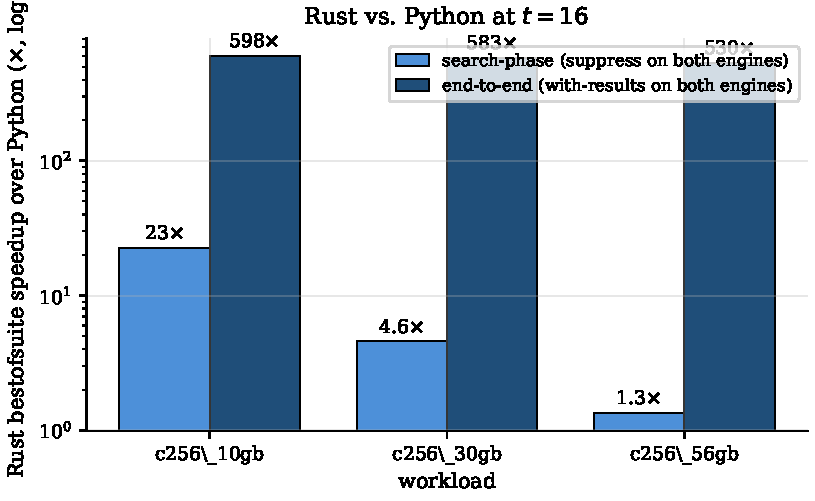
\includegraphics[width=\linewidth]{ch4_e2e_speedup.pdf}
    \column{0.46\textwidth}
    \small
    \begin{tabular}{lrr}
      \toprule
      Workload & search & end-to-end \\
      \midrule
      \texttt{c256\_10gb} & $22.7\times$ & $598\times$ \\
      \texttt{c256\_30gb} & $4.6\times$  & $583\times$ \\
      \texttt{c256\_56gb} & $1.34\times$ & $530\times$ \\
      \bottomrule
    \end{tabular}
    \vspace{1ex}
    \begin{itemize}
      \item End-to-end: 2.4\,h $\to$ 16\,s on the primary workload.
      \item $\sim$99\% of that ratio is avoiding Python's per-(query, cluster) result-dict construction --- \textbf{not} search superiority.
      \item Search phase bends toward the shared hardware ceilings as footprint grows.
    \end{itemize}
  \end{columns}
  \smallskip
  {\small Bonus: the Rust rebinning kernel cuts index-construction alignment by $4.7\times$ (small/medium) and $2.2\times$ (5M histograms).}
\end{frame}

% ---------------------------------------------------------------- 6. Wrap-up
\section{Conclusion}

\begin{frame}{Contributions}
  \begin{enumerate}
    \item \textbf{Rust re-implementation} of Fainder's query pipeline --- bitwise-identical results, $530$--$598\times$ end-to-end, integrated via PyO3. \hfill \emph{engineering}
    \item \textbf{Four-ceiling characterisation} of distribution-aware search on Sapphire Rapids, established via \texttt{perf} counters. \hfill \emph{scientific}
    \item \textbf{Negative-composability pattern}: five independent instances on five axes. \hfill \emph{scientific}
    \item \textbf{Pre-flight ceiling identification}: probe the binding ceiling at the target composition before paying implementation cost. \hfill \emph{methodological}
    \item \textbf{Dispatch-on-regime policy}, validated 23/24 within 5\%, including out-of-distribution. \hfill \emph{engineering}
  \end{enumerate}
  \vfill
  (1) and (5) are the staging ground; (2)--(4) are what generalises.
\end{frame}

\begin{frame}{Takeaway}
  \begin{itemize}
    \item The speedups are specific to this codebase, micro-architecture, and workload.
    \item The structural finding travels: on hardware-near workloads, whether optimisation $B$ helps depends on which ceiling optimisation $A$ has already collected --- invisible to per-operator cost models.
  \end{itemize}
  \vfill
  \begin{alertblock}{One sentence}
    Identify the binding ceiling at the target composition \emph{before} committing the implementation cost of the next optimisation.
  \end{alertblock}
\end{frame}

\begin{frame}[standout]
  Questions?
\end{frame}

% ================================================================ BACKUP
\appendix
\section{Backup}

\begin{frame}{Backup: Why is end-to-end $530\times$ if search is only $1.34\times$?}
  \begin{itemize}
    \item Python's per-(query, cluster) result-dict construction dominates its wall. Measured at $t{=}16$, materialisation accounts for:
    \begin{itemize}
      \item \texttt{c256\_10gb}: $580.9$\,s of $599.7$\,s ($96.9\%$)
      \item \texttt{c256\_30gb}: $1{,}878.5$\,s of $1{,}890.3$\,s ($99.4\%$)
      \item \texttt{c256\_56gb}: $8{,}568$\,s of $8{,}589$\,s ($99.8\%$)
    \end{itemize}
    \item Rust emits results without per-cluster dict churn, so it dodges this cost entirely.
    \item That is why we report both columns: suppress-vs-suppress isolates the search engines; with-results-vs-with-results is what a user experiences.
    \item Both numbers are honest; conflating them would not be.
  \end{itemize}
\end{frame}

\begin{frame}{Backup: Why doesn't f16 win standalone?}
  \begin{itemize}
    \item Prediction: halve the footprint, win in the regime where f32 exceeds L3 but f16 fits.
    \item On \texttt{c256\_56gb} the per-cluster f32 slice ($\sim$105\,KiB) is already L2-resident. Halving it unlocks no new cache-resident regime, but every comparison pays the f16$\to$f32 dequantisation.
    \item Result: no significant standalone win in the 10-rep fine-$t$ sweep; a $+15.6\%$ drag inside the bundle at $t{=}16$.
    \item On \texttt{c1024\_56gb} ($3.2\times$ sparser, $\sim$33\,KiB slices, 610 clusters) the aggregate cluster-loop footprint is the constraint --- there f16 carries $\sim$20\% of the bundle win.
    \item General point: footprint optimisations are density-conditional, not universal.
  \end{itemize}
\end{frame}

\begin{frame}{Backup: Why ``memory-traffic pressure'' and not ``DRAM bandwidth''?}
  \begin{itemize}
    \item STREAM Triad on this machine reaches $\sim$330\,GB/s aggregate.
    \item Accounting the workload's LLC-miss traffic ($64$\,B per missed probe) puts it at $\sim$0.5\% of that peak.
    \item ``Bandwidth-bound'' would claim saturation of the DRAM channels; the counters show nothing close.
    \item What we observe is anti-scaling from aggregate pressure on the on-socket memory subsystem (queues, MLC occupancy, allocator traffic) --- hence \emph{on-socket memory-traffic pressure}.
    \item The naming matters: it predicts which interventions help (fewer bytes per comparison/emit), and that pure bandwidth upgrades would not.
  \end{itemize}
\end{frame}

\begin{frame}{Backup: The local-ids regression --- mechanism}
  \begin{itemize}
    \item \texttt{local-ids} (per-cluster reindexing) was pre-registered as a positive prediction: narrower IDs, less read-side bandwidth.
    \item Measured: \bad{$+186$ to $+245\%$} at $t \in [8, 64]$ on top of \texttt{packed-ids} --- our falsified prediction.
    \item Mechanism, from a direct \texttt{perf stat} probe: the bw$\approx$13 decoder's access pattern over the packed buffer drives the \textbf{dTLB miss rate up $52\times$} per instruction.
    \item TLB-walk stalls ($\sim$100 cycles each) drown the bandwidth saving.
    \item Future work (F1): Transparent Huge Pages (2\,MiB pages) would cut TLB-miss frequency $512\times$ per covered page --- the natural follow-up probe.
  \end{itemize}
\end{frame}

\begin{frame}{Backup: Does any of this generalise beyond one machine?}
  \begin{itemize}
    \item Honest answer: the \emph{thresholds} do not, the \emph{methodology} does.
    \item All experiments ran on one Sapphire Rapids 8468H configuration. Genoa, Granite Rapids, or Grace would shift per-ceiling thresholds and dispatch boundaries.
    \item What transfers: the pre-flight procedure (probe the binding ceiling at the target composition) is machine-agnostic; the four-ceiling taxonomy is a hypothesis set to re-test, not a constant.
    \item Density scope: dispatch is validated between $\sim$8{,}200 and $\sim$26{,}300 hists/cluster; outside that range the policy is a prediction.
    \item Multi-machine deployment would add a fifth candidate ceiling (network), with its own intervention class.
  \end{itemize}
\end{frame}

\begin{frame}{Backup: How was correctness validated?}
  \begin{itemize}
    \item Every Rust build validated \textbf{bitwise-identical} to the Python reference across all workloads: precision $=$ recall $=$ 1.000.
    \item Validation runs in the benchmark harness itself, not as a one-off test --- each measured configuration is also a correctness check.
    \item Rebinning kernel: verified against the Python reference on 200 queries. Rust rounds half-away, NumPy uses banker's rounding; maximum cumulative difference $10^{-4}$ at a handful of rows, no effect on sort order or query results.
    \item Kernel falls back to the Python pipeline if the extension is not importable or for \texttt{cubic\_spline} bin estimation.
  \end{itemize}
\end{frame}

\begin{frame}{Backup: Why Rust, and not C++, Cython, or Numba?}
  \begin{itemize}
    \item The requirement set: no GIL in the hot path, explicit control over layout and allocation, safe shared-memory parallelism, and a maintainable Python integration.
    \item Rust + PyO3 gives all four: Rayon work-stealing without data races, Cargo feature flags to make every ablation a separate reproducible build, and a drop-in extension module for the existing API.
    \item C++ could reach the same performance; the feature-flag ablation matrix and memory safety under 96-thread parallelism are where Rust paid off in practice.
    \item Numba/Cython remove less of the interpreter overhead and keep the allocator and layout decisions in Python's hands --- the layers our measurements show are the actual cost.
  \end{itemize}
\end{frame}

\begin{frame}{Backup: Why does the rebinning speedup drop at 5M histograms?}
  \begin{itemize}
    \item $4.72\times$ (324\,K) and $4.77\times$ (997\,K) drop to $2.18\times$ at 5.02\,M histograms.
    \item Cause: the kernel's own parallelism ceiling --- at that scale it runs at $\sim$2 effective cores of 96, with $\sim$46\% of kernel time on a shared per-cluster allocation.
    \item Not caused by ``NumPy bulk operations dominating'' --- that earlier hypothesis was tested and refuted.
    \item Construction-time cost, paid once per index build; the query-phase findings are unaffected.
  \end{itemize}
\end{frame}

\end{document}
